% !TEX TS-program = pdflatex
% !TEX encoding = UTF-8 Unicode

% This is a simple template for a LaTeX document using the "article" class.
% See "book", "report", "letter" for other types of document.

\documentclass[11pt]{article} % use larger type; default would be 10pt

\usepackage[utf8]{inputenc} % set input encoding (not needed with XeLaTeX)

%%% Examples of Article customizations
% These packages are optional, depending whether you want the features they provide.
% See the LaTeX Companion or other references for full information.

%%% PAGE DIMENSIONS
\usepackage{geometry} % to change the page dimensions
%\geometry{letterpaper} % or letterpaper (US) or a5paper or....
% \geometry{margin=2in} % for example, change the margins to 2 inches all round
% \geometry{landscape} % set up the page for landscape
%   read geometry.pdf for detailed page layout information

\usepackage{graphicx} % support the \includegraphics command and options

% \usepackage[parfill]{parskip} % Activate to begin paragraphs with an empty line rather than an indent

%%% PACKAGES
\usepackage{booktabs} % for much better looking tables
\usepackage{array} % for better arrays (eg matrices) in maths
\usepackage{paralist} % very flexible & customisable lists (eg. enumerate/itemize, etc.)
\usepackage{verbatim} % adds environment for commenting out blocks of text & for better verbatim
\usepackage{subfig} % make it possible to include more than one captioned figure/table in a single float
% These packages are all incorporated in the memoir class to one degree or another...

%%% HEADERS & FOOTERS
\usepackage{fancyhdr} % This should be set AFTER setting up the page geometry
\pagestyle{fancy} % options: empty , plain , fancy
\renewcommand{\headrulewidth}{0pt} % customise the layout...
\lhead{}\chead{}\rhead{}
\lfoot{}\cfoot{\thepage}\rfoot{}

%%% SECTION TITLE APPEARANCE
\usepackage{sectsty}
\allsectionsfont{\sffamily\mdseries\upshape} % (See the fntguide.pdf for font help)
% (This matches ConTeXt defaults)

%%% ToC (table of contents) APPEARANCE
\usepackage[nottoc,notlof,notlot]{tocbibind} % Put the bibliography in the ToC
\usepackage[titles,subfigure]{tocloft} % Alter the style of the Table of Contents
\renewcommand{\cftsecfont}{\rmfamily\mdseries\upshape}
\renewcommand{\cftsecpagefont}{\rmfamily\mdseries\upshape} % No bold!

%%% END Article customizations

%%% The "real" document content comes below...

\title{Project 3}
\author{Alex Cochrane}
%\date{} % Activate to display a given date or no date (if empty),
         % otherwise the current date is printed 

\begin{document}
\maketitle

\section{Abstract}

\paragraph{} The following is a look at a genetic program(GP) evolved to solve the classic Santa Fe Trail problem. First an overview of how I built my GP and how I set up its evolutionary traits will be examined in an easy to read table. This will be referred to later in the discussion section which will talk about problems that arose during the project such as issues with crossover and parents, and a small issue with fitness. The discussion section will also go over the results of the project which are quite mixed. With some of the issues that I had, some of my results were look like the graph in this document. Some however are stagnant and do not change. Prior to the discussion section, are the graphs that show the results and the solutions.
\newline

\begin{tabular}{|l|p{4in}|}
\hline
Algorithm & Generational\\
\hline
Population size & 500\\
\hline
Selection method & Tournament, using an N value of 5\\
\hline
Elitism & Copy the best individual twice\\
\hline
Crossover method & Random node switching between two trees.\\
\hline
Crossover rate & 100\% chance to crossover, 10\% probability of getting a leaf\\
\hline
Mutation method & There was a 2\% probability of mutating a tree. When a tree was selected for mutation, a random node would be given a new type and given new children if needed with a depth of 1 (Terminal into a Non-Terminal for instance).\\
\hline
Operator/non-terminal set & prog2, prog3, if\_food\_ahead\\
\hline
Terminal set & Forward, Left, Right\\
\hline
Fitness function & Amount of food eaten. Maximization problem.\\
\hline
\end{tabular}

\pagebreak
\begin{center}
Fitness Graph
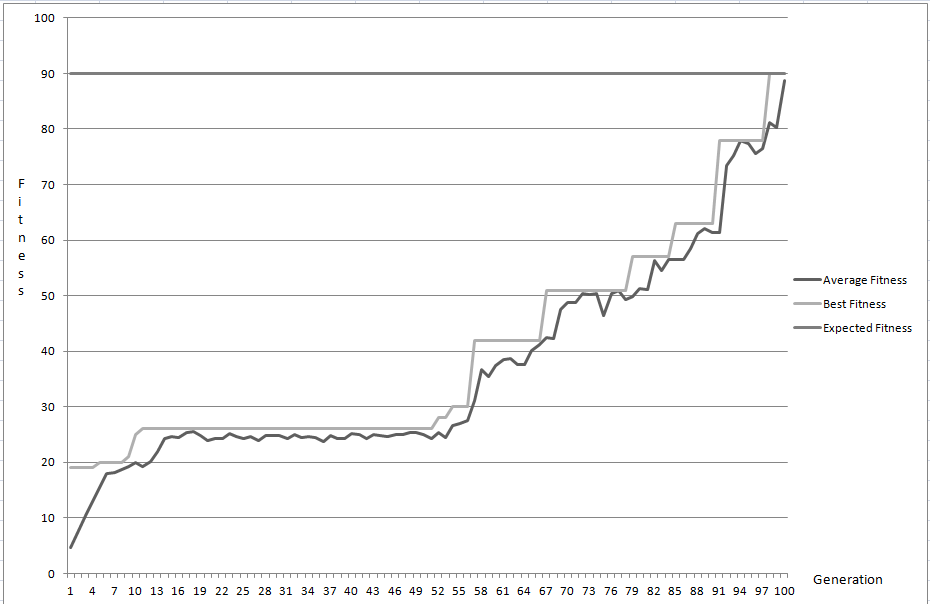
\includegraphics[scale = 0.65]{Fitness_Graph}
\end{center}

\paragraph{Best Evolved Path} To best show that path that was evolved I though it would be best to show a starting graph and then a graph that represents the final solution. The graph is very simple in its representation. A 1 is food, a 2 is where an ant ate food, and a 3 is where an ant moved but did not find any food. The first graph is of a typical best solution at generation 0. It has found roughly 15 pieces of food which is my typical starting best fitness. The second graph however is at generation 100 for possibly my best solution that I ever ran. I have not been able to replicate this solutions ability to get to 90 even with its long stretch of being stuck around 25 pieces of food. The biggest behaviour that I can see being favored here is that it likes tries to search over one space left and right of the last location it found food. It seems to move left or right and then move forward checking to see if there is food to its left or right and then switching sides if not and repeating until it hits food again.

\pagebreak
\begin{center}
Generation 0:
\begin{verbatim}
2 2 1 1 3 3 3           3 3 3 3                                 
  3 3 2 3                                                       
      1                                           1 1 1         
      1                                         1         1     
      1                                         1         1     
      1 1 1 1   1 1 1 1 1                 1 1                   
                        1                                 1     
                        1                                       
                        1               1                       
                        1               1                 1     
                        1               1                       
                                        1                       
                        1                                 1     
                        1                                       
                        1               1           1 1 1       
                        1               1     1                 
                                  1                             
                                1                               
                        1       1               1               
                        1       1                     1         
                        1         3 3 3 3                       
                        1     3 2 3     3                       
                        1     3         3 3         1           
        3 3 3 3         1     3           3   1                 
      1 2     2 2 2 1 1       3 1         3                     
  1     3 3 3 3 3 3             1     3 3 3                     
  1             3 3             2 3 3 3                         
  1             2 2 2 2 1 1 1   3                               
3 2 3       3 2 3     3         3 3                             
3   3       3 1       3           3                             
3   2 1 1 1 3         3 3         3                             
3 3 3       3           3     3 3 3                             
\end{verbatim}
\end{center}

\pagebreak
\begin{center}
Generation 100:
\begin{verbatim}
2 2 2 2                                                         
      2                                                 3 3 3   
      2                                         3 2 2 2 3   3   
      2                                         2         2 3   
      2                                       3 2         2     
      2 2 2 2 3 2 2 2 2 2             3 3 2 2 3           3     
                        2             3                   2     
                        2             3 3               3 3     
                        2               2               3       
                        2               2               3 2     
                        2               2               3 3     
                        3               2               3       
                        2               3               3 2     
                        2               3     3 3 3     3 3     
                        2               3     3   3 2 2 2       
                        2           3 3 2     2                 
                      3 3       3 2 3                           
                      3         2                               
                      3 2       2   3 3 3 3   3 2 3 3 3         
                        2       2 3 3     3 3 3       2         
                        2         3 3 3 3   3 3 3 3   3         
                        2     3 2 3     3   3     3   3         
                        2     3         3 3 3 3   3 2 3         
3 3 3   3 3 3           2     3 3         3   2                 
3   3 2 2   3 2 2 2 2 2 3       2         3 3 3                 
3 2                             2                               
  2           3 3               2 3                             
  2           3 2 2 2 2 2 2 2 3   3                             
  2           2               3 3 3                             
3 3           2 3                                               
3   2 2 2 2 3   3                                               
3 3 3       3 3 3                                               
\end{verbatim}
\end{center}
\pagebreak

\section{Discussion}

\paragraph{Issues} Some issues that I ran into, starting from the simplest to the most complicated, consisted of fitness not improving and crossover losing parents. To start with fitness not improving, I noticed that even with the ant being allowed to move 600 times, he would continually make it about 30 squares and stop. The problem was I was saying the ant moved on non-terminals even though I only wanted them to be able to move and count against movement during a terminal.

\paragraph{} The issue with crossover is a lot more complicated and I was not able to solve but just create a workaround. Every once in awhile during crossover, which is the only reason why I keep track of parents, a parent will not be set and I can perform crossover. When this happens, I ignore this crossover. If this error appears later, like in a copy where I need to know the parent to move it into the new tree, I reset the tree and create a new non corrupt tree. This is not an ideal situation but, because this is never my best solution and it is typically a solution that has been used in crossover many times and will most likely not be selected in the next generation, it is as ideal as it can be and does not seem to affect the end result.

\paragraph{Results} As stated before, the results were quite mixed in their performance. Sometimes trees would conform too quickly and get stuck at a lackluster fitness. Occasionally, with about a 10\% probability, I would get a solution that looked like what I have shown in the prior graph. The average fitness therefore for 100 different runs of the GP would be somewhere around 30. This is because most fitnesses would plateau out at 20 to 25 in fitness for the runs. The ones that did not get stuck in this plateau eventually reach somewhere from 70 to 90 in fitness.

\paragraph{} The last thing to point out about my results is that even though I have an issue with crossover. When it is working, it works quite dependably. This can be seen in each generation as the size of trees is constantly changing. The protective hypothesis is obviously present because when observing some of these trees, situations with multiple nested loops appear or with a left and right directly following each other in multiple spots. This analysis of the trees shows that my crossover is doing what it was built to do but some corruption in my parent nodes has created problems that in the end don't seem to be that detrimental to the end result of the GP.

\end{document}
